\documentclass[letterpaper,spanish]{letter}
\usepackage[T1]{fontenc}
\usepackage[utf8]{inputenc}
\usepackage[spanish]{babel}
\usepackage{lmodern}
\usepackage{marvosym}
\usepackage{amsmath}
\usepackage{amsfonts}
\usepackage{amssymb}
\usepackage{graphicx}

\address{Germ\'{a}n Avenda\~{n}o Ram\'{i}rez\\ \Email ~iedabgerman@autistici.org}
\signature{Germ\'{a}n Avenda\~{n}o Ram\'{i}rez\\C.C. 79'003 541 de Guaduas Cund.\\Lic. U.D. M.Sc. U.N.}
\date{14 de agosto de 2018}

\begin{document}

\begin{letter}{ANDREY ALÍ ALVÁREZ GAITÁN\\Rector\\COLEGIO ARBORIZADORA BAJA I.E.D.}
	
\opening{Cordial saludo}
Solicito para el próximo jueves 16 de agosto, el medio día compensatorio por haber votado en las elecciones en la segunda vuelta presidencial y el otro medio día por haberme transportado por 30 días en bicicleta al trabajo según la ley 1811 de 2016, para participar como candidato en las elecciones a la Asamblea de nuestra cooperativa Codema. Los días que me transporté para llegar y salir del trabajo y que uso para solicitar mi medio día compensado son:

Abril: 6, 16-19, 24-27, 30; Mayo: 2-4, 7-8, 11, 15-18, 21-25; Julio: 17,19 31; Agosto: 8, 10.

\begin{center}
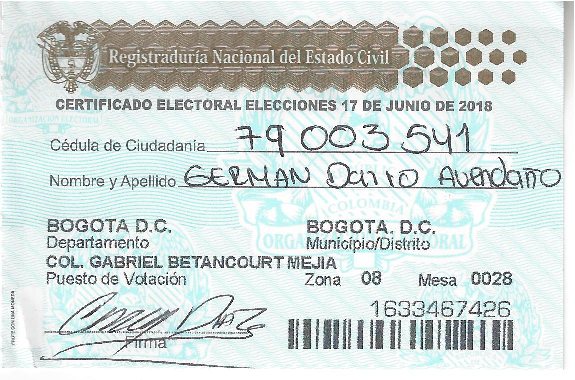
\includegraphics[scale=1]{Images/Compensatorio.pdf} 
\end{center}

\closing{Atentamente,}

%cc{}
%\ps{PS: PostScriptum}
%\encl{Listado de adjuntos}

\end{letter}
\end{document}
